\begin{enumerate}[label=\thesection.\arabic*,ref=\thesection.\theenumi]
\numberwithin{equation}{enumi}
\numberwithin{figure}{enumi}
\numberwithin{table}{enumi}
\item Draw a right triangle ${ABC}$ in which $BC=12$ cm, $AB=5$ cm and $\angle{B}=90\degree$.
\item Draw an isosceles triangle ${ABC}$ in which $AB$=$AC$=6 cm and $BC$ =6 cm.
\item Draw a triangle ${ABC}$ in which $AB$=5 cm. $BC=6 cm\text{ and }\angle {ABC}=60\degree$.
\item Draw a triangle ${ABC}$ in which $AB$=4 cm, $BC=6 cm\text{ and }AC=9$
\item Draw a triangle ${ABC}$ in which $BC=6$ cm, $CA=5$ cm and $AB=4$ cm. 
\item Draw a parallelogram ${ABCD}$ in which $BC=5$ cm, $AB=3$ cm and $\angle{ABC}=60\degree$, divide it into triangles ${ACB}\text{ and }{ABD}$ by the diagonal $BD$. 
\item In triangles ABC and PQR, $ \angle{A} = \angle{Q} $ and $ \angle{B} = \angle{R} $.Which side of $ \triangle{PQR} $ should be equal to side AB of $ \triangle{ABC} $ so that the two triangles are congruent?Give reason for your answer.

\item In triangles ABC and PQR, $ \angle{A} = \angle{Q} $ and $ \angle{B} = \angle{R} $.Which side of $ \triangle{PQR} $should be equal to side BC of $ \triangle{ABC} $ so that the two triangles are congruent?Give reason for your answer.

\item "If two sides and an angle of one triangle are equal to two sides and an angle ofanother triangle,then two triangles must be congruent."Is the statement true?Why?

\item "If two angles and a side one triangle are equal to two angles and a side of another triangle,then the two triangles must be congruent."Is the statement true?Why?

\item Is it possible to construct a triangle with lengths of its sides as 4 cm, 3 cm and 7 cm?Give reason for your answer.

\item It is given that $ \triangle{ABC} \cong \triangle{RPQ} $.Is it true to say that BC = QR?Why?

\item If $ \triangle{PQR} \cong \triangle{EDF} $,then is it true to say that PR = EF?Give reason for your answer.

\item In $ \triangle{PQR} $,$ \angle{P} = 70\degree $ and $ \angle{R} = 30\degree $.Which side of the triangle is the longest?Give reason for your answer.

\item AD is a median of the triangle ABC.Is it true that AB + BC + CA $ > $ 2AD?Give reason for your answer.

\item M is a point on side BC of a triangle ABC such that AM is the bisector of $ \angle{BAC} $.Is it true to say that perimeter of the triangle is greater than 2AM?Give reason for your answer.

\item Is it possible to construct a triangle with lengths of its sides as 9 cm, 7 cm and 17 cm?Give reason for your answer.

\item Is it possible to cosntruct a triangle with lengths of its sides as 8 cm, 7 cm and 4 cm?Give reason for your answer.

	\item $\vec{ABC}$ is an isosceles triangle with $\vec{AB=AC}$ and $\vec{BD}$ and $\vec{CE}$ are its two medians. Show that $\vec{BD=CE}$.
	\item In Fig. \ref{fig:exemplar/9.7.37.3.2}, $\vec{D}$ and $\vec{E}$ are the points on side $\vec{BC}$ of a $\triangle \vec{ABC}$ such that $\vec{BD=CE}$ and $\vec{AD=AE}$. Show that $\triangle \vec{ABD} \cong \triangle \vec{ACE}$.
\begin{figure}[h]
	\centering
	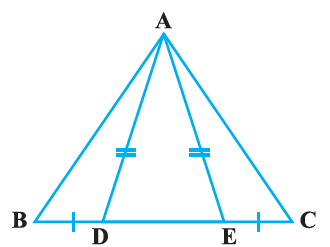
\includegraphics[width=\columnwidth]{exemplar/9.7.3/figs/Figure1.png}
	\caption{}
	\label{fig:exemplar/9.7.37.3.2}
\end{figure}
\item $\vec{CDE}$ is an equilateral triangle formed on a side $\vec{CD}$ of a square $\vec{ABCD}$ (Fig. \ref{fig:exemplar/9.7.37.3.3}). Show that $\triangle \vec{ADE} \cong \triangle \vec{BCE}$.
\begin{figure}[h]
	\centering
	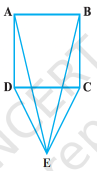
\includegraphics[width=\columnwidth]{exemplar/9.7.3/figs/Figure2.png}
	\caption{}
	\label{fig:exemplar/9.7.37.3.3}
\end{figure}
\item In Fig. \ref{fig:exemplar/9.7.37.3.4}, $\vec{BA} \perp \vec{AC}$, $\vec{DE} \perp \vec{DF}$ such that $\vec{BA=DE}$ and $\vec{BF=EC}$. Show that $\triangle \vec{ABC} \cong \triangle \vec{DEF}$.
\begin{figure}[h]
	\centering
	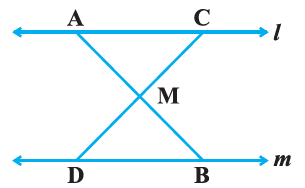
\includegraphics[width=\columnwidth]{exemplar/9.7.3/figs/Figure3.png}
	\caption{}
	\label{fig:exemplar/9.7.37.3.4}
\end{figure}
\item $\vec{Q}$ is a point on the side $\vec{SR}$ of $\triangle \vec{PSR}$ such that $\vec{PQ=PR}$. Prove that $\vec{PS>PQ}$.
\item $\vec{S}$ is any point on side $\vec{QR}$ of a $\triangle \vec{PQR}$. Show that $\vec{PQ+QR+RP>2PS}$.
\item $\vec{D}$ is any point on side $\vec{AC}$ of a $\triangle \vec{ABC}$ with $\vec{AB=AC}$. Show that $\vec{CD<BD}$.
\item In Fig. \ref{fig:exemplar/9.7.37.3.8}, $\vec{l} \| \vec{m}$ an $\vec{M}$ is the mid-point of a line segment $\vec{AB}$. Show that $\vec{M}$ is also the mid-point of any line segment $\vec{CD}$, having its end points on $\vec{l}$ and $\vec{m}$, respectively.
\begin{figure}[h]
	\centering
	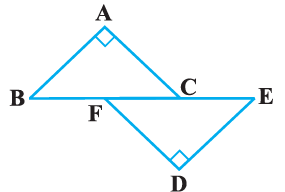
\includegraphics[width=\columnwidth]{exemplar/9.7.3/figs/Figure4.png}
	\caption{}
	\label{fig:exemplar/9.7.37.3.8}
\end{figure}
\item Bisectors of the $\angle \vec{B}$ and $\angle \vec{C}$ of an isosceles triangle with $\vec{AB=AC}$ intersect each other at $\vec{O}$. $\vec{BO}$ is produced to a point $\vec{M}$. Prove that $\angle \vec{MOC}= \angle \vec{ABC}$.
\item Bisectors of the $\angle \vec{B}$ and $\angle \vec{C}$ of an isosceles triangle $\vec{ABC}$ with $\vec{AB=AC}$ intersect each other at $\vec{O}$. Show that the external angle adjacent to $\angle \vec{ABC}$ is equal to $\angle \vec{BOC}$.
\item In Fig. \ref{fig:exemplar/9.7.37.3.11}, $\vec{AD}$ is the bisector of $\angle \vec{BAC}$. Prove that $\vec{AB>BD}$.
\begin{figure}[h]
	\centering
	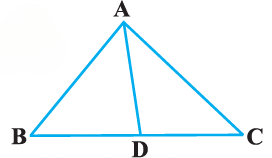
\includegraphics[width=\columnwidth]{exemplar/9.7.3/figs/Figure5.png}
	\caption{}
	\label{fig:exemplar/9.7.37.3.11}
\end{figure}
\item Find all the angles of an equilateral triangle.
%\item The image of an object placed at a point $A$ before a plane mirror $LM$ is seen at the point $B$ by an observer at $D$ as shown in \eqref{fig:exemplar/9.7.4Figure 1} Prove that the image is as far behind the mirror as the object is in front  of the mirror.
%
%[\textcolor{cyan}{Hint:} $CN$ is normal to the mirror. Also, angle of incidence = angle of reflection].
%\begin{figure}[!h]
%\centering
% \includegraphics[width=\columnwidth]{./exemplar/9.7.4/figs/7A.png}
%\caption{}
%\label{fig:exemplar/9.7.4Figure 1}
%\end{figure}
\item $P$ is a point on the bisector of $\angle ABC$. If the line through $P$, parallel to $BA$ meet $BC$ at $Q$, prove that $BPQ$ is an isosceles triangle.
\item $ABC$ is a right triangle with $AB = AC$. Bisector of $\angle A$ meets $BC$ at $D$. Prove that $BC = 2 AD$
\item $ABC$ and $DBC$ are two triangles on the same base $BC$ such that $A$ and $D$ lie on the opposite sides of $BC$, $AB = AC$ and $DB = DC$. Show that $AD$ is the perpendicular bisector of BC.
\item ABC is an isosceles triangle in which $AC = BC$. $AD$ and $BE$ are respectively two altitudes to sides $BC$ and $AC$. Prove that $AE = BD$.
\item Prove that sum of any two sides of a triangle is greater than twice the median with respect to the third side.
\item In a triangle $ABC$, $D$ is the mid-point of side $AC$ such that $ BD = \frac{1}{2} AC $. Show that $\angle ABC$ is a right angle.
\item In a right triangle, prove that the line-segment joining the mid-point of the hypotenuse to the opposite vertex is half the hypotenuse.
\item Two lines $l$ and $m$ intersect at the point $O$ and $P$ is a point on a line $n$ passing through the point $O$ such that $P$ is equidistant from $l$ and $m$. Prove that $n$ is the bisector of the angle formed by $l$ and $m$.
\item $ABC$ is a right triangle such that $AB = AC$ and bisector of angle $C$ intersects the side $AB$ at $D$. Prove that $AC + AD = BC$.
\item Prove that in a triangle, other than an equilateral triangle, angle opposite the longest side is greater than $\frac{2}{3}$ of a right angle.
\end{enumerate}
